\documentclass[titlepage]{article}
\usepackage[tc]{titlepic}
\usepackage{graphicx}
\usepackage{amsmath}
\usepackage[top=25mm, bottom=25mm, left=27mm, right=27mm]{geometry}
\usepackage{caption}
\usepackage{listings}
\usepackage{lstlangarm}
\usepackage{tabu}
\usepackage[outdir=./]{epstopdf}


\date{}
\author{Erdal Sidal Dogan\\ \#041702023  \and Alp
	Gokcek \\ \#041701014}
\title{
\includegraphics[width=0.6\textwidth]{../images/logo_en_color.png}\\ 
\vspace{5em}
EE306 - Microprocessors\\
\vspace{2em}
\textbf{Laboratory Exercise 3 \linebreak Subroutines
}\\
\vspace{1.5em}
March 17, 2020}

\begin{document}
	\maketitle
	\section{Part III - Sigma Sum}
	In this experiment we wrote an assembly program that finds the mean of given set of numbers, length of the number sequence is defined as $N$. Listing \ref{part3code} below calculates the result of the following expression $\sum_{i=0}^{N}i$
	
	\lstinputlisting[language={[ARM]Assembler}, frame=single, basicstyle=\ttfamily, caption=Assembly Code for Sigma sum \& calculating average]{../source_codes/task-iii.s} \label{part3code}
	
	\begin{figure}[h]
		\centering
		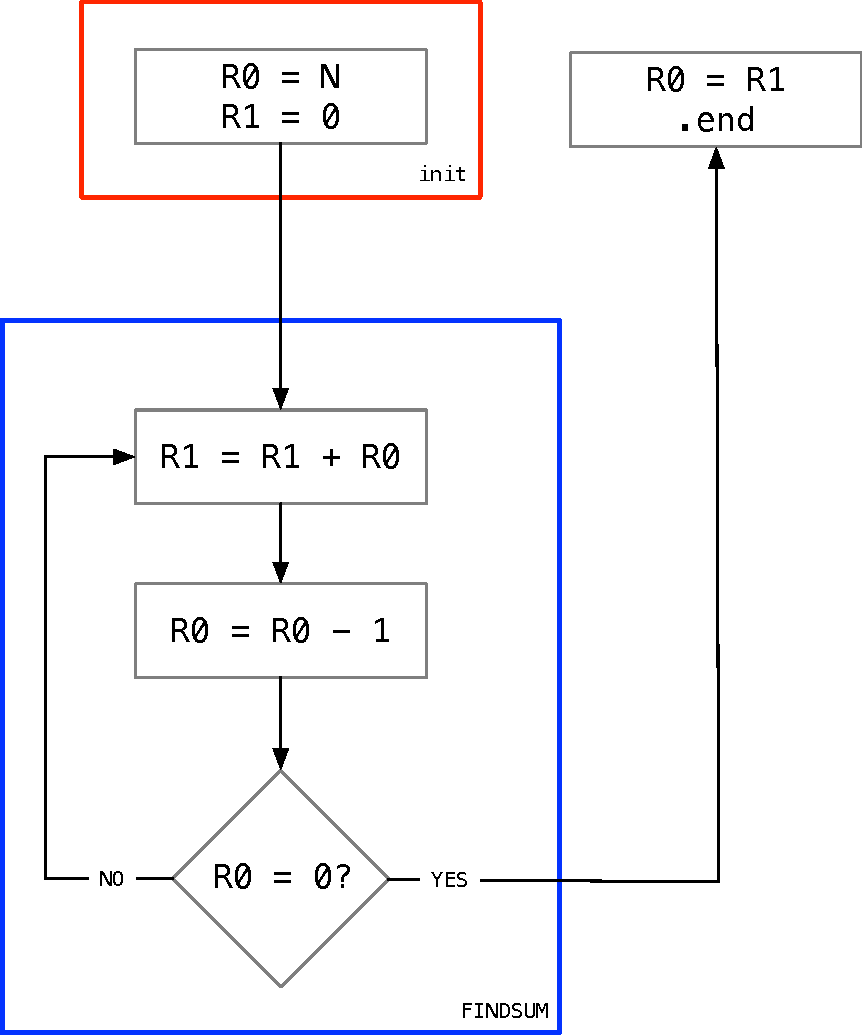
\includegraphics[scale=.5]{../images/task-iii.pdf}
		\caption{Flowchart of the Listing \ref{part3code}}
	\end{figure}
	
	\section{Part IV - Bubble Sort}
	Bubble sort explanation
	\lstinputlisting[language={[ARM]Assembler}, frame=single, basicstyle=\ttfamily, caption= Assembly code for bubble sort algorithm]{../source_codes/task-iv.s}
	

\end{document}